% Sloczynski (2022) formal apparatus, cut from northwestern_day2_cunningham.tex
% (Aug 2026, referee2 round 1). Linear projections, tau_APLE, Theorem 1,
% Assumptions 1-4, Corollary 1 and its proof.
% To restore: % Sloczynski (2022) formal apparatus, cut from northwestern_day2_cunningham.tex
% (Aug 2026, referee2 round 1). Linear projections, tau_APLE, Theorem 1,
% Assumptions 1-4, Corollary 1 and its proof.
% To restore: % Sloczynski (2022) formal apparatus, cut from northwestern_day2_cunningham.tex
% (Aug 2026, referee2 round 1). Linear projections, tau_APLE, Theorem 1,
% Assumptions 1-4, Corollary 1 and its proof.
% To restore: % Sloczynski (2022) formal apparatus, cut from northwestern_day2_cunningham.tex
% (Aug 2026, referee2 round 1). Linear projections, tau_APLE, Theorem 1,
% Assumptions 1-4, Corollary 1 and its proof.
% To restore: \input{sloczynski_formal_cut.tex}
\begin{frame}
\frametitle{Main Result: Algebra of OLS and Descriptive Estimands}
\begin{itemize}
    \item Focuses on the algebra of OLS and descriptive estimands.
    \item Potential outcomes and conditions for causal interpretation discussed in Section IIC.
    \item Main result does not require causal interpretation assumptions.
\end{itemize}
\end{frame}

\begin{frame}{Linear projection}

\begin{itemize}
\item Linear projection is a concept from the theory of linear regression describing the expected value of the dependent variable as a linear function of independent variables 
\item It does not necessarily incorporate randomness or an error term and so should be considered distinct from the ``data generating process'' which does
\item It posits a relationship that says, "If we knew the true parameters, this is how we would expect Y to change, on average, with changes in X and D"
\end{itemize}

\end{frame}

\begin{frame}
\frametitle{Linear Projection}
\begin{itemize}
    \item Let \( L(\cdot | \cdot) \) denote the linear projection.
    \item Interested in the interpretation of \( \tau \) in the linear projection of \( y \) on \( d \) and \( X \):
    \[ L(y | 1, d, X) = \alpha + \tau d + X\beta \quad \text{(2)} \]
    \item This projection is distinct from the structural conditional mean.
\end{itemize}
\end{frame}

\begin{frame}
\frametitle{Probability of Treatment and Propensity Score}
\begin{itemize}
    \item The unconditional probability of treatment:
    \[ \rho = P(d = 1) \quad \text{(3)} \]
    \item Propensity score from the linear probability model:
    \[ p(X) = L(d | 1, X) = \alpha_p + X\beta_p \quad \text{(4)} \]
    \item \( p(X) \) is the best linear approximation to the true propensity score.
    \item Equations (2) and (4) provide the specification.
\end{itemize}
\end{frame}

\begin{frame}
\frametitle{Flexibility of the Linear Projection}
\begin{itemize}
    \item Equation (2) can be seen as partially linear, including powers and cross-products of control variables.
    \item The propensity score approximation can be made very accurate.
\end{itemize}
\end{frame}

\begin{frame}
\frametitle{Linear Projections with Propensity Score}
\begin{itemize}
    \item Separate linear projections of \( y \) on \( p(X) \) for \( d = 1 \) and \( d = 0 \):
    \[ L[y | 1, p(X), d = 1] = \alpha_1 + \gamma_1 \times p(X) \quad \text{(5)} \]
    \[ L[y | 1, p(X), d = 0] = \alpha_0 + \gamma_0 \times p(X) \quad \text{(6)} \]
    \item Definitions are based on the variability of the propensity score within treatment groups.
\end{itemize}
\end{frame}

\begin{frame}
\frametitle{Assumptions for Linear Projections}
\begin{itemize}
    \item Assumption 1: Existence and uniqueness of linear projections in (2) and (4).
    \item Assumption 2: Existence and uniqueness of linear projections in (5) and (6).
    \item These assumptions guarantee the linear projections are well-defined and unique.
    \item Both of these assumptions (fn. 3) are generally innocuous although the second one rules out a small number of interesting applications like regression adjustments in completely randomized experiments -- but in these cases OLS will estimate the ATE consistently (Imbens and Rubin 2015)
\end{itemize}
\end{frame}

\begin{frame}
\frametitle{Defining Average Partial Linear Effects}
\begin{itemize}
    \item The average partial linear effect of \( d \):
    \[ \tau_{\text{APLE}} = (\alpha_1 - \alpha_0) + (\gamma_1 - \gamma_0) \times E[p(X)] \quad \text{(7)} \]
    \item The average partial linear effect of \( d \) on group \( j \) (where \( j = 0, 1 \)):
    \[ \tau_{\text{APLE}, j} = (\alpha_1 - \alpha_0) + (\gamma_1 - \gamma_0) \times E[p(X) | d = j] \quad \text{(8)} \]
    \item These estimands are well-defined under Assumptions 1 and 2.
\end{itemize}
\end{frame}

\begin{frame}
\frametitle{Causal Interpretation and Theorem 1}
\begin{itemize}
    \item Causal interpretation requires additional assumptions beyond 1 and 2.
    \item Theorem 1 is more general, relying only on Assumptions 1 and 2.
    \item It applies to the algebraic properties of OLS estimators.
\end{itemize}
\end{frame}

\begin{frame}
\frametitle{Weighted Average Interpretation of OLS (Theorem 1)}

Under assumptions (1) and (2)

$$\tau = \omega_1 \times \tau_{APLE,1} + \omega_0 \times \tau_{APLE,0}$$
 
 where the weights are equal to:
 
\begin{align*}
\omega_1 &= \frac{(1-\rho) \times V[p(X)|d=0]}{\rho \times V[p(X)|d=1] + (1-\rho) \times V[p(X)|d=0]} \\
\text{and} \quad \omega_0 &= 1 - \omega_1
\end{align*}

\end{frame}

\begin{frame}
\frametitle{Theorem 1: Interpretation of the OLS Estimand}
\begin{itemize}
    \item The OLS estimand \( \tau \) is a convex combination of \( \tau_{\text{APLE},1} \) and \( \tau_{\text{APLE},0} \).
    \item Reflects the weighted average outcome of a three-step procedure:
    \begin{enumerate}
        \item Obtain the propensity score \( p(X) \).
        \item Calculate \( \tau_{\text{APLE},1} \) and \( \tau_{\text{APLE},0} \) for \( d = 1 \) and \( d = 0 \) via linear projections.
        \item Compute the weighted average of \( \tau_{\text{APLE},1} \) and \( \tau_{\text{APLE},0} \).
    \end{enumerate}
\end{itemize}
\end{frame}

\begin{frame}
\frametitle{Weighting in the Estimation of \( \tau \)}
\begin{itemize}
    \item The weight on \( \tau_{\text{APLE},1} \), \( \omega_1 \), decreases with \( V[p(X) | d = 1] \) and the probability of treatment \( \rho \).
    \item Conversely, the weight on \( \tau_{\text{APLE},0} \), \( \omega_0 \), increases with \( V[p(X) | d = 1] \) and \( \rho \).
    \item The weighting scheme implies that larger groups receive less weight on their respective \( \tau_{\text{APLE},j} \).
\end{itemize}
\end{frame}

\begin{frame}{Assumptions for an Illustrative Example}
    The following graph shows how the weight on \( \tau_{\text{APLE},1} \) decreases as the variance of the propensity score among the treated increases using the following simplifications for illustrative purposes:
    \begin{itemize}
        \item The variance among the non-treated \( V[p(X) | d = 0] \) is constant at 0.1.
        \item The probability of treatment \( \rho \) is 0.5, meaning that half of the population is treated.
        \item The variance among the treated \( V[p(X) | d = 1] \) varies from 0.1 to 0.9 for the purpose of the illustration.
    \end{itemize}
\end{frame}

\begin{frame}{Weight on \( \tau_{\text{APLE},1} \) with Varying Variance among Treated}
    \begin{figure}
        \centering
        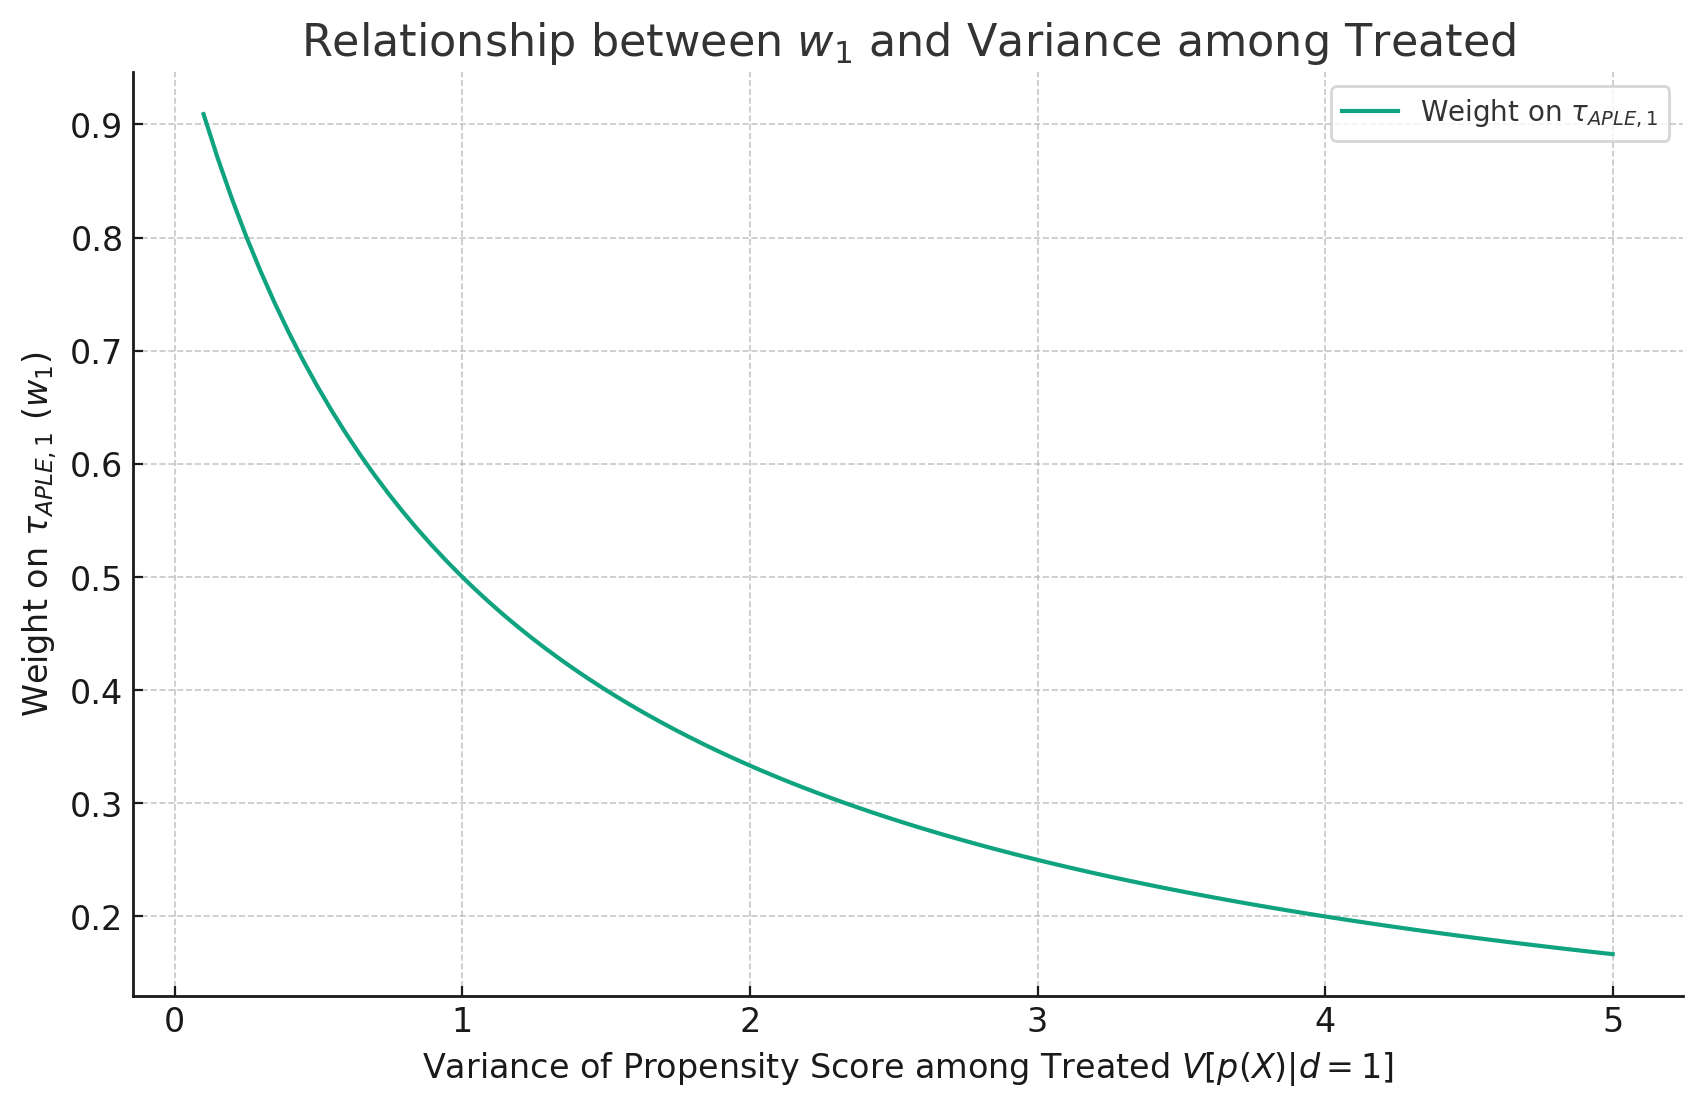
\includegraphics[width=0.8\textwidth]{./lecture_includes/tymon_variance_weight.png}
        \caption{The relationship between the weight \( \omega_1 \) on \( \tau_{\text{APLE},1} \) and the variance of the propensity score among the treated \( V[p(X) | d = 1] \). As the variance among the treated increases, the weight on \( \tau_{\text{APLE},1} \) decreases.}
    \end{figure}
\end{frame}

\begin{frame}{Causal Interpretation of OLS}
  Theorem 1 ("Weighted Average Interpretation of OLS") is general due to its reliance solely on the existence and uniqueness of linear projections; however, for a causal interpretation of OLS, we must introduce:
  \begin{itemize}
    \item Potential outcomes \( y(1) \) and \( y(0) \) instead of realized outcomes
    \item Defined causal parameters: ATE, ATT, and ATU
    \item Introduce assumptions that will ensure a causal interpretation of \( \tau \)
  \end{itemize}
\end{frame}

\begin{frame}{Assumption 3 for Causal Interpretation}
  \begin{block}{Unconfoundedness in Mean Potential Outcomes or "Ignorability in Means"}
    \begin{enumerate}
      \item \( E [y(1) | X, d] = E[y(1) | X] \)
      \item \( E[y(0) | X, d] = E[y(0) | X] \)
    \end{enumerate}
  \end{block}
  Assumptions 3 is our standard unconfoundedness assumption but limited to means (slightly weaker but it's all we need)
\end{frame}

\begin{frame}{Assumption 4 for Causal Interpretation}
  \begin{block}{Linearity in Potential Outcomes}
    Assumption 4 posits that the conditional expectations of potential outcomes are linear in the propensity score:
    \begin{enumerate}
      \item \( E[y(1) | X] = \alpha_1 + \gamma_1 \times p(X) \)
      \item \( E[y(0) | X] = \alpha_0 + \gamma_0 \times p(X) \)
    \end{enumerate}
  \end{block}
\end{frame}

\begin{frame}{Historical and Practical Context of Assumption 4}
  While not a common assumption, it is not necessarily strong due to:
  \begin{itemize}
    \item The flexibility in the specification of \( X \), which can include nonlinear terms.
    \item The automatic satisfaction of this assumption in saturated models.
  \end{itemize}

    The linearity assumption has historical roots and practical implications:
    \begin{itemize}
      \item Historically aligned with Rosenbaum and Rubin (1983).
      \item Assumed linearity of \( E[d | X] \) in several notable econometric works.
      \item It is restrictive but can be mitigated by model specification choices.
    \end{itemize}
\end{frame}

\begin{frame}[shrink]{Corollary 1: Causal Interpretation of OLS}
  Under assumptions the first two linear projection related assumptions and these two new causal assumptions, then
  \[
    \tau = \omega_1 \times \tau_{\text{ATT}} + \omega_0 \times \tau_{\text{ATU}}
  \]
  
  In words, this states that under those four assumptions, the OLS weights from theorem 1 apply to the causal parameters we care about, the ATT and the ATU, and so therefore $\tau$ has a causal interpretation.  
  
  \bigskip
  
  But there's a catch: the greater the proportion of treated units, the smaller the OLS weight on the ATT, which is a problem given ATE = $\rho \times ATT + (1-\rho) ATU$
\end{frame}

\begin{frame}[shrink]{Proving Corollary 1 with Assumptions 3 and 4}
  \begin{itemize}
    \item Assumption 3 (Unconfoundedness) allows us to estimate the ATE using realized outcomes, as the expected potential outcomes are equal to the observed outcomes conditional on covariates \( X \):
    \[ E[y(1) - y(0) | X] = E[y | X, d = 1] - E[y | X, d = 0] \]
    \item Assumption 4 specifies the functional form of the expected potential outcomes as linear in the propensity score:
    \[ E[y(1) | X] = \alpha_1 + \gamma_1 \times p(X), \quad E[y(0) | X] = \alpha_0 + \gamma_0 \times p(X) \]
    \item Together, they imply that the OLS estimand for the treated (\( \tau_{\text{ATT}} \)) and untreated (\( \tau_{\text{ATU}} \)) equates to the Average Partial Linear Effects (APLE):
    \[ \tau_{\text{ATT}} = \tau_{\text{APLE},1}, \quad \tau_{\text{ATU}} = \tau_{\text{APLE},0} \]
    \item This connects the causal treatment effects (ATT and ATU) directly to the estimated effects from the linear projections.
  \end{itemize}
\end{frame}

\begin{frame}
\frametitle{Main Result: Algebra of OLS and Descriptive Estimands}
\begin{itemize}
    \item Focuses on the algebra of OLS and descriptive estimands.
    \item Potential outcomes and conditions for causal interpretation discussed in Section IIC.
    \item Main result does not require causal interpretation assumptions.
\end{itemize}
\end{frame}

\begin{frame}{Linear projection}

\begin{itemize}
\item Linear projection is a concept from the theory of linear regression describing the expected value of the dependent variable as a linear function of independent variables 
\item It does not necessarily incorporate randomness or an error term and so should be considered distinct from the ``data generating process'' which does
\item It posits a relationship that says, "If we knew the true parameters, this is how we would expect Y to change, on average, with changes in X and D"
\end{itemize}

\end{frame}

\begin{frame}
\frametitle{Linear Projection}
\begin{itemize}
    \item Let \( L(\cdot | \cdot) \) denote the linear projection.
    \item Interested in the interpretation of \( \tau \) in the linear projection of \( y \) on \( d \) and \( X \):
    \[ L(y | 1, d, X) = \alpha + \tau d + X\beta \quad \text{(2)} \]
    \item This projection is distinct from the structural conditional mean.
\end{itemize}
\end{frame}

\begin{frame}
\frametitle{Probability of Treatment and Propensity Score}
\begin{itemize}
    \item The unconditional probability of treatment:
    \[ \rho = P(d = 1) \quad \text{(3)} \]
    \item Propensity score from the linear probability model:
    \[ p(X) = L(d | 1, X) = \alpha_p + X\beta_p \quad \text{(4)} \]
    \item \( p(X) \) is the best linear approximation to the true propensity score.
    \item Equations (2) and (4) provide the specification.
\end{itemize}
\end{frame}

\begin{frame}
\frametitle{Flexibility of the Linear Projection}
\begin{itemize}
    \item Equation (2) can be seen as partially linear, including powers and cross-products of control variables.
    \item The propensity score approximation can be made very accurate.
\end{itemize}
\end{frame}

\begin{frame}
\frametitle{Linear Projections with Propensity Score}
\begin{itemize}
    \item Separate linear projections of \( y \) on \( p(X) \) for \( d = 1 \) and \( d = 0 \):
    \[ L[y | 1, p(X), d = 1] = \alpha_1 + \gamma_1 \times p(X) \quad \text{(5)} \]
    \[ L[y | 1, p(X), d = 0] = \alpha_0 + \gamma_0 \times p(X) \quad \text{(6)} \]
    \item Definitions are based on the variability of the propensity score within treatment groups.
\end{itemize}
\end{frame}

\begin{frame}
\frametitle{Assumptions for Linear Projections}
\begin{itemize}
    \item Assumption 1: Existence and uniqueness of linear projections in (2) and (4).
    \item Assumption 2: Existence and uniqueness of linear projections in (5) and (6).
    \item These assumptions guarantee the linear projections are well-defined and unique.
    \item Both of these assumptions (fn. 3) are generally innocuous although the second one rules out a small number of interesting applications like regression adjustments in completely randomized experiments -- but in these cases OLS will estimate the ATE consistently (Imbens and Rubin 2015)
\end{itemize}
\end{frame}

\begin{frame}
\frametitle{Defining Average Partial Linear Effects}
\begin{itemize}
    \item The average partial linear effect of \( d \):
    \[ \tau_{\text{APLE}} = (\alpha_1 - \alpha_0) + (\gamma_1 - \gamma_0) \times E[p(X)] \quad \text{(7)} \]
    \item The average partial linear effect of \( d \) on group \( j \) (where \( j = 0, 1 \)):
    \[ \tau_{\text{APLE}, j} = (\alpha_1 - \alpha_0) + (\gamma_1 - \gamma_0) \times E[p(X) | d = j] \quad \text{(8)} \]
    \item These estimands are well-defined under Assumptions 1 and 2.
\end{itemize}
\end{frame}

\begin{frame}
\frametitle{Causal Interpretation and Theorem 1}
\begin{itemize}
    \item Causal interpretation requires additional assumptions beyond 1 and 2.
    \item Theorem 1 is more general, relying only on Assumptions 1 and 2.
    \item It applies to the algebraic properties of OLS estimators.
\end{itemize}
\end{frame}

\begin{frame}
\frametitle{Weighted Average Interpretation of OLS (Theorem 1)}

Under assumptions (1) and (2)

$$\tau = \omega_1 \times \tau_{APLE,1} + \omega_0 \times \tau_{APLE,0}$$
 
 where the weights are equal to:
 
\begin{align*}
\omega_1 &= \frac{(1-\rho) \times V[p(X)|d=0]}{\rho \times V[p(X)|d=1] + (1-\rho) \times V[p(X)|d=0]} \\
\text{and} \quad \omega_0 &= 1 - \omega_1
\end{align*}

\end{frame}

\begin{frame}
\frametitle{Theorem 1: Interpretation of the OLS Estimand}
\begin{itemize}
    \item The OLS estimand \( \tau \) is a convex combination of \( \tau_{\text{APLE},1} \) and \( \tau_{\text{APLE},0} \).
    \item Reflects the weighted average outcome of a three-step procedure:
    \begin{enumerate}
        \item Obtain the propensity score \( p(X) \).
        \item Calculate \( \tau_{\text{APLE},1} \) and \( \tau_{\text{APLE},0} \) for \( d = 1 \) and \( d = 0 \) via linear projections.
        \item Compute the weighted average of \( \tau_{\text{APLE},1} \) and \( \tau_{\text{APLE},0} \).
    \end{enumerate}
\end{itemize}
\end{frame}

\begin{frame}
\frametitle{Weighting in the Estimation of \( \tau \)}
\begin{itemize}
    \item The weight on \( \tau_{\text{APLE},1} \), \( \omega_1 \), decreases with \( V[p(X) | d = 1] \) and the probability of treatment \( \rho \).
    \item Conversely, the weight on \( \tau_{\text{APLE},0} \), \( \omega_0 \), increases with \( V[p(X) | d = 1] \) and \( \rho \).
    \item The weighting scheme implies that larger groups receive less weight on their respective \( \tau_{\text{APLE},j} \).
\end{itemize}
\end{frame}

\begin{frame}{Assumptions for an Illustrative Example}
    The following graph shows how the weight on \( \tau_{\text{APLE},1} \) decreases as the variance of the propensity score among the treated increases using the following simplifications for illustrative purposes:
    \begin{itemize}
        \item The variance among the non-treated \( V[p(X) | d = 0] \) is constant at 0.1.
        \item The probability of treatment \( \rho \) is 0.5, meaning that half of the population is treated.
        \item The variance among the treated \( V[p(X) | d = 1] \) varies from 0.1 to 0.9 for the purpose of the illustration.
    \end{itemize}
\end{frame}

\begin{frame}{Weight on \( \tau_{\text{APLE},1} \) with Varying Variance among Treated}
    \begin{figure}
        \centering
        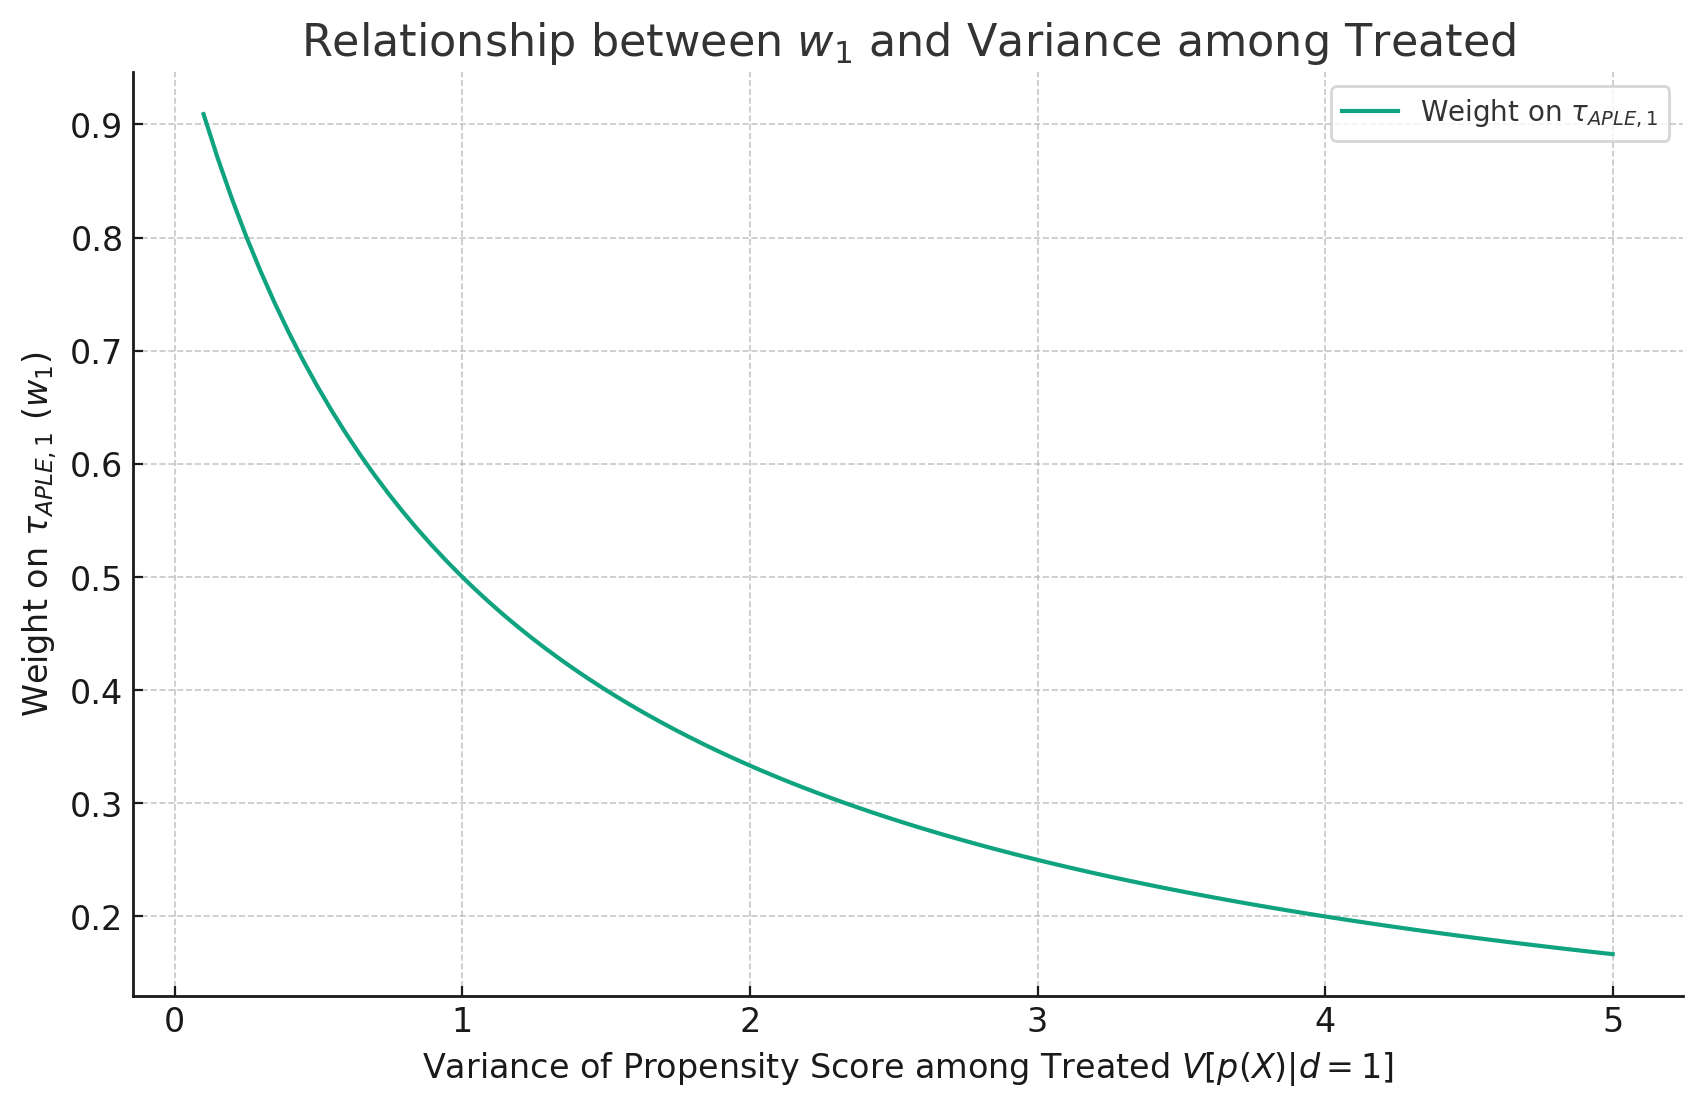
\includegraphics[width=0.8\textwidth]{./lecture_includes/tymon_variance_weight.png}
        \caption{The relationship between the weight \( \omega_1 \) on \( \tau_{\text{APLE},1} \) and the variance of the propensity score among the treated \( V[p(X) | d = 1] \). As the variance among the treated increases, the weight on \( \tau_{\text{APLE},1} \) decreases.}
    \end{figure}
\end{frame}

\begin{frame}{Causal Interpretation of OLS}
  Theorem 1 ("Weighted Average Interpretation of OLS") is general due to its reliance solely on the existence and uniqueness of linear projections; however, for a causal interpretation of OLS, we must introduce:
  \begin{itemize}
    \item Potential outcomes \( y(1) \) and \( y(0) \) instead of realized outcomes
    \item Defined causal parameters: ATE, ATT, and ATU
    \item Introduce assumptions that will ensure a causal interpretation of \( \tau \)
  \end{itemize}
\end{frame}

\begin{frame}{Assumption 3 for Causal Interpretation}
  \begin{block}{Unconfoundedness in Mean Potential Outcomes or "Ignorability in Means"}
    \begin{enumerate}
      \item \( E [y(1) | X, d] = E[y(1) | X] \)
      \item \( E[y(0) | X, d] = E[y(0) | X] \)
    \end{enumerate}
  \end{block}
  Assumptions 3 is our standard unconfoundedness assumption but limited to means (slightly weaker but it's all we need)
\end{frame}

\begin{frame}{Assumption 4 for Causal Interpretation}
  \begin{block}{Linearity in Potential Outcomes}
    Assumption 4 posits that the conditional expectations of potential outcomes are linear in the propensity score:
    \begin{enumerate}
      \item \( E[y(1) | X] = \alpha_1 + \gamma_1 \times p(X) \)
      \item \( E[y(0) | X] = \alpha_0 + \gamma_0 \times p(X) \)
    \end{enumerate}
  \end{block}
\end{frame}

\begin{frame}{Historical and Practical Context of Assumption 4}
  While not a common assumption, it is not necessarily strong due to:
  \begin{itemize}
    \item The flexibility in the specification of \( X \), which can include nonlinear terms.
    \item The automatic satisfaction of this assumption in saturated models.
  \end{itemize}

    The linearity assumption has historical roots and practical implications:
    \begin{itemize}
      \item Historically aligned with Rosenbaum and Rubin (1983).
      \item Assumed linearity of \( E[d | X] \) in several notable econometric works.
      \item It is restrictive but can be mitigated by model specification choices.
    \end{itemize}
\end{frame}

\begin{frame}[shrink]{Corollary 1: Causal Interpretation of OLS}
  Under assumptions the first two linear projection related assumptions and these two new causal assumptions, then
  \[
    \tau = \omega_1 \times \tau_{\text{ATT}} + \omega_0 \times \tau_{\text{ATU}}
  \]
  
  In words, this states that under those four assumptions, the OLS weights from theorem 1 apply to the causal parameters we care about, the ATT and the ATU, and so therefore $\tau$ has a causal interpretation.  
  
  \bigskip
  
  But there's a catch: the greater the proportion of treated units, the smaller the OLS weight on the ATT, which is a problem given ATE = $\rho \times ATT + (1-\rho) ATU$
\end{frame}

\begin{frame}[shrink]{Proving Corollary 1 with Assumptions 3 and 4}
  \begin{itemize}
    \item Assumption 3 (Unconfoundedness) allows us to estimate the ATE using realized outcomes, as the expected potential outcomes are equal to the observed outcomes conditional on covariates \( X \):
    \[ E[y(1) - y(0) | X] = E[y | X, d = 1] - E[y | X, d = 0] \]
    \item Assumption 4 specifies the functional form of the expected potential outcomes as linear in the propensity score:
    \[ E[y(1) | X] = \alpha_1 + \gamma_1 \times p(X), \quad E[y(0) | X] = \alpha_0 + \gamma_0 \times p(X) \]
    \item Together, they imply that the OLS estimand for the treated (\( \tau_{\text{ATT}} \)) and untreated (\( \tau_{\text{ATU}} \)) equates to the Average Partial Linear Effects (APLE):
    \[ \tau_{\text{ATT}} = \tau_{\text{APLE},1}, \quad \tau_{\text{ATU}} = \tau_{\text{APLE},0} \]
    \item This connects the causal treatment effects (ATT and ATU) directly to the estimated effects from the linear projections.
  \end{itemize}
\end{frame}

\begin{frame}
\frametitle{Main Result: Algebra of OLS and Descriptive Estimands}
\begin{itemize}
    \item Focuses on the algebra of OLS and descriptive estimands.
    \item Potential outcomes and conditions for causal interpretation discussed in Section IIC.
    \item Main result does not require causal interpretation assumptions.
\end{itemize}
\end{frame}

\begin{frame}{Linear projection}

\begin{itemize}
\item Linear projection is a concept from the theory of linear regression describing the expected value of the dependent variable as a linear function of independent variables 
\item It does not necessarily incorporate randomness or an error term and so should be considered distinct from the ``data generating process'' which does
\item It posits a relationship that says, "If we knew the true parameters, this is how we would expect Y to change, on average, with changes in X and D"
\end{itemize}

\end{frame}

\begin{frame}
\frametitle{Linear Projection}
\begin{itemize}
    \item Let \( L(\cdot | \cdot) \) denote the linear projection.
    \item Interested in the interpretation of \( \tau \) in the linear projection of \( y \) on \( d \) and \( X \):
    \[ L(y | 1, d, X) = \alpha + \tau d + X\beta \quad \text{(2)} \]
    \item This projection is distinct from the structural conditional mean.
\end{itemize}
\end{frame}

\begin{frame}
\frametitle{Probability of Treatment and Propensity Score}
\begin{itemize}
    \item The unconditional probability of treatment:
    \[ \rho = P(d = 1) \quad \text{(3)} \]
    \item Propensity score from the linear probability model:
    \[ p(X) = L(d | 1, X) = \alpha_p + X\beta_p \quad \text{(4)} \]
    \item \( p(X) \) is the best linear approximation to the true propensity score.
    \item Equations (2) and (4) provide the specification.
\end{itemize}
\end{frame}

\begin{frame}
\frametitle{Flexibility of the Linear Projection}
\begin{itemize}
    \item Equation (2) can be seen as partially linear, including powers and cross-products of control variables.
    \item The propensity score approximation can be made very accurate.
\end{itemize}
\end{frame}

\begin{frame}
\frametitle{Linear Projections with Propensity Score}
\begin{itemize}
    \item Separate linear projections of \( y \) on \( p(X) \) for \( d = 1 \) and \( d = 0 \):
    \[ L[y | 1, p(X), d = 1] = \alpha_1 + \gamma_1 \times p(X) \quad \text{(5)} \]
    \[ L[y | 1, p(X), d = 0] = \alpha_0 + \gamma_0 \times p(X) \quad \text{(6)} \]
    \item Definitions are based on the variability of the propensity score within treatment groups.
\end{itemize}
\end{frame}

\begin{frame}
\frametitle{Assumptions for Linear Projections}
\begin{itemize}
    \item Assumption 1: Existence and uniqueness of linear projections in (2) and (4).
    \item Assumption 2: Existence and uniqueness of linear projections in (5) and (6).
    \item These assumptions guarantee the linear projections are well-defined and unique.
    \item Both of these assumptions (fn. 3) are generally innocuous although the second one rules out a small number of interesting applications like regression adjustments in completely randomized experiments -- but in these cases OLS will estimate the ATE consistently (Imbens and Rubin 2015)
\end{itemize}
\end{frame}

\begin{frame}
\frametitle{Defining Average Partial Linear Effects}
\begin{itemize}
    \item The average partial linear effect of \( d \):
    \[ \tau_{\text{APLE}} = (\alpha_1 - \alpha_0) + (\gamma_1 - \gamma_0) \times E[p(X)] \quad \text{(7)} \]
    \item The average partial linear effect of \( d \) on group \( j \) (where \( j = 0, 1 \)):
    \[ \tau_{\text{APLE}, j} = (\alpha_1 - \alpha_0) + (\gamma_1 - \gamma_0) \times E[p(X) | d = j] \quad \text{(8)} \]
    \item These estimands are well-defined under Assumptions 1 and 2.
\end{itemize}
\end{frame}

\begin{frame}
\frametitle{Causal Interpretation and Theorem 1}
\begin{itemize}
    \item Causal interpretation requires additional assumptions beyond 1 and 2.
    \item Theorem 1 is more general, relying only on Assumptions 1 and 2.
    \item It applies to the algebraic properties of OLS estimators.
\end{itemize}
\end{frame}

\begin{frame}
\frametitle{Weighted Average Interpretation of OLS (Theorem 1)}

Under assumptions (1) and (2)

$$\tau = \omega_1 \times \tau_{APLE,1} + \omega_0 \times \tau_{APLE,0}$$
 
 where the weights are equal to:
 
\begin{align*}
\omega_1 &= \frac{(1-\rho) \times V[p(X)|d=0]}{\rho \times V[p(X)|d=1] + (1-\rho) \times V[p(X)|d=0]} \\
\text{and} \quad \omega_0 &= 1 - \omega_1
\end{align*}

\end{frame}

\begin{frame}
\frametitle{Theorem 1: Interpretation of the OLS Estimand}
\begin{itemize}
    \item The OLS estimand \( \tau \) is a convex combination of \( \tau_{\text{APLE},1} \) and \( \tau_{\text{APLE},0} \).
    \item Reflects the weighted average outcome of a three-step procedure:
    \begin{enumerate}
        \item Obtain the propensity score \( p(X) \).
        \item Calculate \( \tau_{\text{APLE},1} \) and \( \tau_{\text{APLE},0} \) for \( d = 1 \) and \( d = 0 \) via linear projections.
        \item Compute the weighted average of \( \tau_{\text{APLE},1} \) and \( \tau_{\text{APLE},0} \).
    \end{enumerate}
\end{itemize}
\end{frame}

\begin{frame}
\frametitle{Weighting in the Estimation of \( \tau \)}
\begin{itemize}
    \item The weight on \( \tau_{\text{APLE},1} \), \( \omega_1 \), decreases with \( V[p(X) | d = 1] \) and the probability of treatment \( \rho \).
    \item Conversely, the weight on \( \tau_{\text{APLE},0} \), \( \omega_0 \), increases with \( V[p(X) | d = 1] \) and \( \rho \).
    \item The weighting scheme implies that larger groups receive less weight on their respective \( \tau_{\text{APLE},j} \).
\end{itemize}
\end{frame}

\begin{frame}{Assumptions for an Illustrative Example}
    The following graph shows how the weight on \( \tau_{\text{APLE},1} \) decreases as the variance of the propensity score among the treated increases using the following simplifications for illustrative purposes:
    \begin{itemize}
        \item The variance among the non-treated \( V[p(X) | d = 0] \) is constant at 0.1.
        \item The probability of treatment \( \rho \) is 0.5, meaning that half of the population is treated.
        \item The variance among the treated \( V[p(X) | d = 1] \) varies from 0.1 to 0.9 for the purpose of the illustration.
    \end{itemize}
\end{frame}

\begin{frame}{Weight on \( \tau_{\text{APLE},1} \) with Varying Variance among Treated}
    \begin{figure}
        \centering
        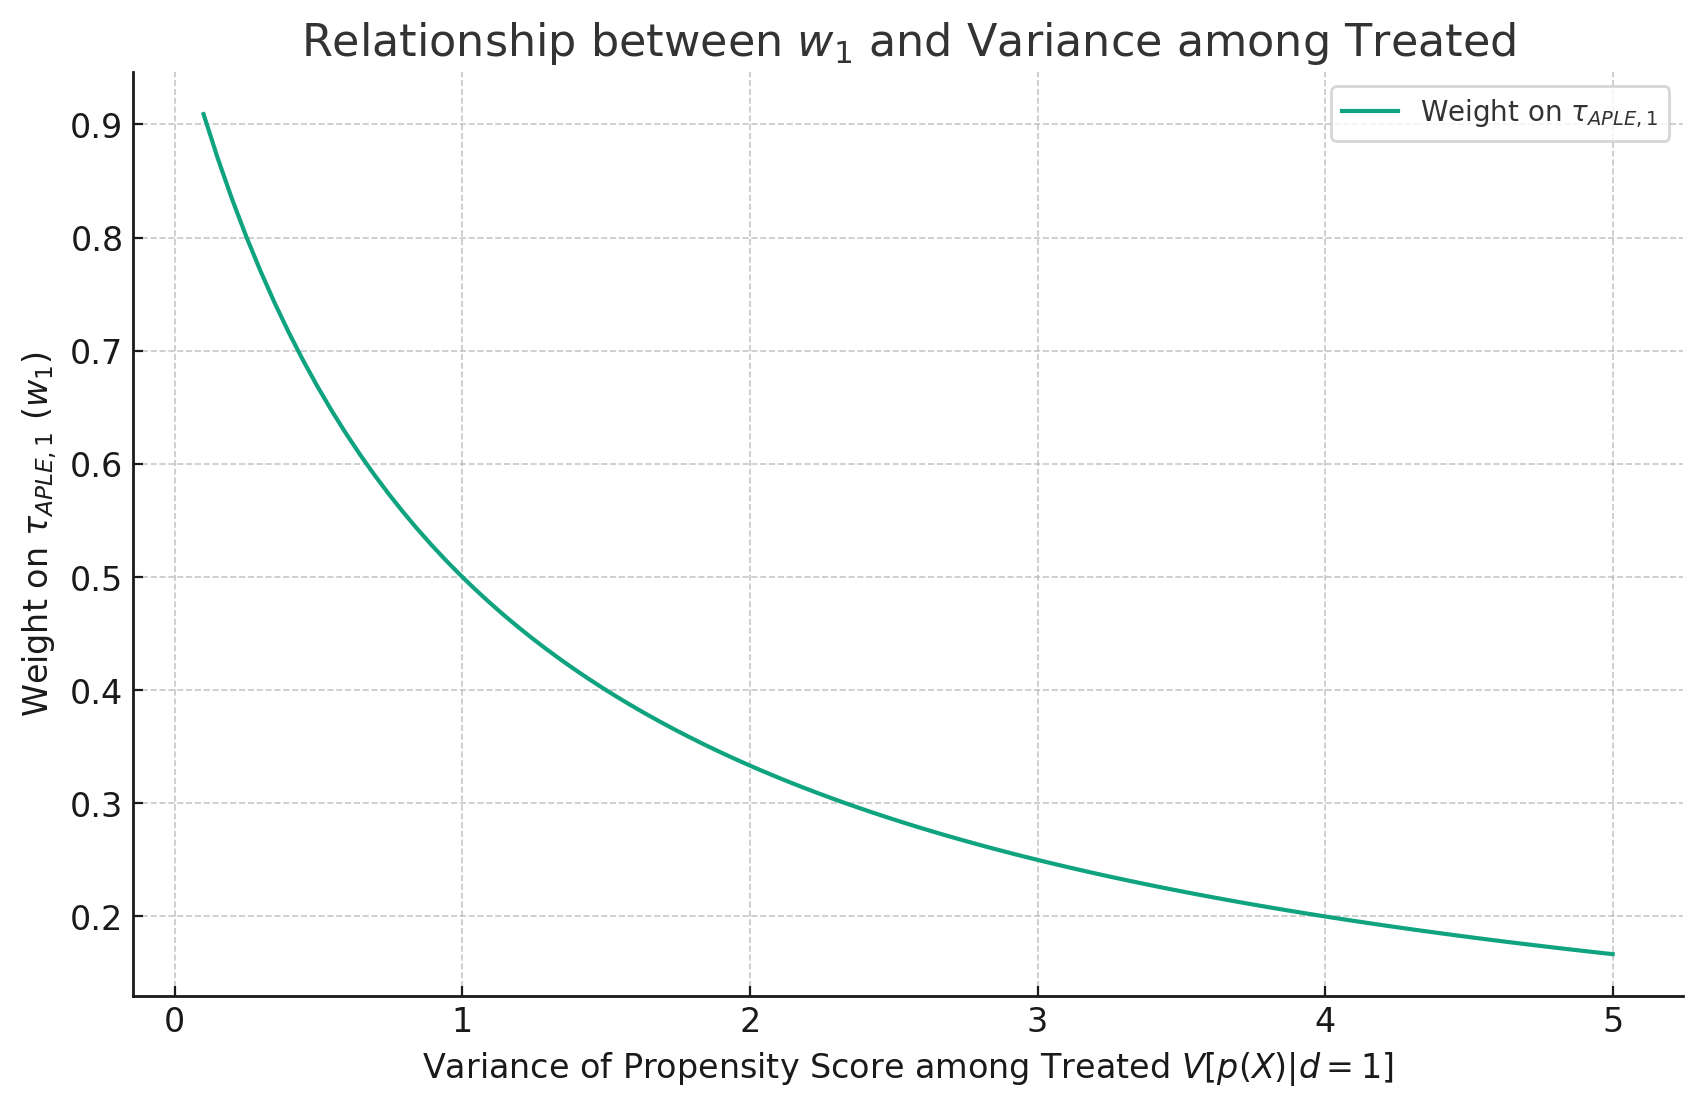
\includegraphics[width=0.8\textwidth]{./lecture_includes/tymon_variance_weight.png}
        \caption{The relationship between the weight \( \omega_1 \) on \( \tau_{\text{APLE},1} \) and the variance of the propensity score among the treated \( V[p(X) | d = 1] \). As the variance among the treated increases, the weight on \( \tau_{\text{APLE},1} \) decreases.}
    \end{figure}
\end{frame}

\begin{frame}{Causal Interpretation of OLS}
  Theorem 1 ("Weighted Average Interpretation of OLS") is general due to its reliance solely on the existence and uniqueness of linear projections; however, for a causal interpretation of OLS, we must introduce:
  \begin{itemize}
    \item Potential outcomes \( y(1) \) and \( y(0) \) instead of realized outcomes
    \item Defined causal parameters: ATE, ATT, and ATU
    \item Introduce assumptions that will ensure a causal interpretation of \( \tau \)
  \end{itemize}
\end{frame}

\begin{frame}{Assumption 3 for Causal Interpretation}
  \begin{block}{Unconfoundedness in Mean Potential Outcomes or "Ignorability in Means"}
    \begin{enumerate}
      \item \( E [y(1) | X, d] = E[y(1) | X] \)
      \item \( E[y(0) | X, d] = E[y(0) | X] \)
    \end{enumerate}
  \end{block}
  Assumptions 3 is our standard unconfoundedness assumption but limited to means (slightly weaker but it's all we need)
\end{frame}

\begin{frame}{Assumption 4 for Causal Interpretation}
  \begin{block}{Linearity in Potential Outcomes}
    Assumption 4 posits that the conditional expectations of potential outcomes are linear in the propensity score:
    \begin{enumerate}
      \item \( E[y(1) | X] = \alpha_1 + \gamma_1 \times p(X) \)
      \item \( E[y(0) | X] = \alpha_0 + \gamma_0 \times p(X) \)
    \end{enumerate}
  \end{block}
\end{frame}

\begin{frame}{Historical and Practical Context of Assumption 4}
  While not a common assumption, it is not necessarily strong due to:
  \begin{itemize}
    \item The flexibility in the specification of \( X \), which can include nonlinear terms.
    \item The automatic satisfaction of this assumption in saturated models.
  \end{itemize}

    The linearity assumption has historical roots and practical implications:
    \begin{itemize}
      \item Historically aligned with Rosenbaum and Rubin (1983).
      \item Assumed linearity of \( E[d | X] \) in several notable econometric works.
      \item It is restrictive but can be mitigated by model specification choices.
    \end{itemize}
\end{frame}

\begin{frame}[shrink]{Corollary 1: Causal Interpretation of OLS}
  Under assumptions the first two linear projection related assumptions and these two new causal assumptions, then
  \[
    \tau = \omega_1 \times \tau_{\text{ATT}} + \omega_0 \times \tau_{\text{ATU}}
  \]
  
  In words, this states that under those four assumptions, the OLS weights from theorem 1 apply to the causal parameters we care about, the ATT and the ATU, and so therefore $\tau$ has a causal interpretation.  
  
  \bigskip
  
  But there's a catch: the greater the proportion of treated units, the smaller the OLS weight on the ATT, which is a problem given ATE = $\rho \times ATT + (1-\rho) ATU$
\end{frame}

\begin{frame}[shrink]{Proving Corollary 1 with Assumptions 3 and 4}
  \begin{itemize}
    \item Assumption 3 (Unconfoundedness) allows us to estimate the ATE using realized outcomes, as the expected potential outcomes are equal to the observed outcomes conditional on covariates \( X \):
    \[ E[y(1) - y(0) | X] = E[y | X, d = 1] - E[y | X, d = 0] \]
    \item Assumption 4 specifies the functional form of the expected potential outcomes as linear in the propensity score:
    \[ E[y(1) | X] = \alpha_1 + \gamma_1 \times p(X), \quad E[y(0) | X] = \alpha_0 + \gamma_0 \times p(X) \]
    \item Together, they imply that the OLS estimand for the treated (\( \tau_{\text{ATT}} \)) and untreated (\( \tau_{\text{ATU}} \)) equates to the Average Partial Linear Effects (APLE):
    \[ \tau_{\text{ATT}} = \tau_{\text{APLE},1}, \quad \tau_{\text{ATU}} = \tau_{\text{APLE},0} \]
    \item This connects the causal treatment effects (ATT and ATU) directly to the estimated effects from the linear projections.
  \end{itemize}
\end{frame}

\begin{frame}
\frametitle{Main Result: Algebra of OLS and Descriptive Estimands}
\begin{itemize}
    \item Focuses on the algebra of OLS and descriptive estimands.
    \item Potential outcomes and conditions for causal interpretation discussed in Section IIC.
    \item Main result does not require causal interpretation assumptions.
\end{itemize}
\end{frame}

\begin{frame}{Linear projection}

\begin{itemize}
\item Linear projection is a concept from the theory of linear regression describing the expected value of the dependent variable as a linear function of independent variables 
\item It does not necessarily incorporate randomness or an error term and so should be considered distinct from the ``data generating process'' which does
\item It posits a relationship that says, "If we knew the true parameters, this is how we would expect Y to change, on average, with changes in X and D"
\end{itemize}

\end{frame}

\begin{frame}
\frametitle{Linear Projection}
\begin{itemize}
    \item Let \( L(\cdot | \cdot) \) denote the linear projection.
    \item Interested in the interpretation of \( \tau \) in the linear projection of \( y \) on \( d \) and \( X \):
    \[ L(y | 1, d, X) = \alpha + \tau d + X\beta \quad \text{(2)} \]
    \item This projection is distinct from the structural conditional mean.
\end{itemize}
\end{frame}

\begin{frame}
\frametitle{Probability of Treatment and Propensity Score}
\begin{itemize}
    \item The unconditional probability of treatment:
    \[ \rho = P(d = 1) \quad \text{(3)} \]
    \item Propensity score from the linear probability model:
    \[ p(X) = L(d | 1, X) = \alpha_p + X\beta_p \quad \text{(4)} \]
    \item \( p(X) \) is the best linear approximation to the true propensity score.
    \item Equations (2) and (4) provide the specification.
\end{itemize}
\end{frame}

\begin{frame}
\frametitle{Flexibility of the Linear Projection}
\begin{itemize}
    \item Equation (2) can be seen as partially linear, including powers and cross-products of control variables.
    \item The propensity score approximation can be made very accurate.
\end{itemize}
\end{frame}

\begin{frame}
\frametitle{Linear Projections with Propensity Score}
\begin{itemize}
    \item Separate linear projections of \( y \) on \( p(X) \) for \( d = 1 \) and \( d = 0 \):
    \[ L[y | 1, p(X), d = 1] = \alpha_1 + \gamma_1 \times p(X) \quad \text{(5)} \]
    \[ L[y | 1, p(X), d = 0] = \alpha_0 + \gamma_0 \times p(X) \quad \text{(6)} \]
    \item Definitions are based on the variability of the propensity score within treatment groups.
\end{itemize}
\end{frame}

\begin{frame}
\frametitle{Assumptions for Linear Projections}
\begin{itemize}
    \item Assumption 1: Existence and uniqueness of linear projections in (2) and (4).
    \item Assumption 2: Existence and uniqueness of linear projections in (5) and (6).
    \item These assumptions guarantee the linear projections are well-defined and unique.
    \item Both of these assumptions (fn. 3) are generally innocuous although the second one rules out a small number of interesting applications like regression adjustments in completely randomized experiments -- but in these cases OLS will estimate the ATE consistently (Imbens and Rubin 2015)
\end{itemize}
\end{frame}

\begin{frame}
\frametitle{Defining Average Partial Linear Effects}
\begin{itemize}
    \item The average partial linear effect of \( d \):
    \[ \tau_{\text{APLE}} = (\alpha_1 - \alpha_0) + (\gamma_1 - \gamma_0) \times E[p(X)] \quad \text{(7)} \]
    \item The average partial linear effect of \( d \) on group \( j \) (where \( j = 0, 1 \)):
    \[ \tau_{\text{APLE}, j} = (\alpha_1 - \alpha_0) + (\gamma_1 - \gamma_0) \times E[p(X) | d = j] \quad \text{(8)} \]
    \item These estimands are well-defined under Assumptions 1 and 2.
\end{itemize}
\end{frame}

\begin{frame}
\frametitle{Causal Interpretation and Theorem 1}
\begin{itemize}
    \item Causal interpretation requires additional assumptions beyond 1 and 2.
    \item Theorem 1 is more general, relying only on Assumptions 1 and 2.
    \item It applies to the algebraic properties of OLS estimators.
\end{itemize}
\end{frame}

\begin{frame}
\frametitle{Weighted Average Interpretation of OLS (Theorem 1)}

Under assumptions (1) and (2)

$$\tau = \omega_1 \times \tau_{APLE,1} + \omega_0 \times \tau_{APLE,0}$$
 
 where the weights are equal to:
 
\begin{align*}
\omega_1 &= \frac{(1-\rho) \times V[p(X)|d=0]}{\rho \times V[p(X)|d=1] + (1-\rho) \times V[p(X)|d=0]} \\
\text{and} \quad \omega_0 &= 1 - \omega_1
\end{align*}

\end{frame}

\begin{frame}
\frametitle{Theorem 1: Interpretation of the OLS Estimand}
\begin{itemize}
    \item The OLS estimand \( \tau \) is a convex combination of \( \tau_{\text{APLE},1} \) and \( \tau_{\text{APLE},0} \).
    \item Reflects the weighted average outcome of a three-step procedure:
    \begin{enumerate}
        \item Obtain the propensity score \( p(X) \).
        \item Calculate \( \tau_{\text{APLE},1} \) and \( \tau_{\text{APLE},0} \) for \( d = 1 \) and \( d = 0 \) via linear projections.
        \item Compute the weighted average of \( \tau_{\text{APLE},1} \) and \( \tau_{\text{APLE},0} \).
    \end{enumerate}
\end{itemize}
\end{frame}

\begin{frame}
\frametitle{Weighting in the Estimation of \( \tau \)}
\begin{itemize}
    \item The weight on \( \tau_{\text{APLE},1} \), \( \omega_1 \), decreases with \( V[p(X) | d = 1] \) and the probability of treatment \( \rho \).
    \item Conversely, the weight on \( \tau_{\text{APLE},0} \), \( \omega_0 \), increases with \( V[p(X) | d = 1] \) and \( \rho \).
    \item The weighting scheme implies that larger groups receive less weight on their respective \( \tau_{\text{APLE},j} \).
\end{itemize}
\end{frame}

\begin{frame}{Assumptions for an Illustrative Example}
    The following graph shows how the weight on \( \tau_{\text{APLE},1} \) decreases as the variance of the propensity score among the treated increases using the following simplifications for illustrative purposes:
    \begin{itemize}
        \item The variance among the non-treated \( V[p(X) | d = 0] \) is constant at 0.1.
        \item The probability of treatment \( \rho \) is 0.5, meaning that half of the population is treated.
        \item The variance among the treated \( V[p(X) | d = 1] \) varies from 0.1 to 0.9 for the purpose of the illustration.
    \end{itemize}
\end{frame}

\begin{frame}{Weight on \( \tau_{\text{APLE},1} \) with Varying Variance among Treated}
    \begin{figure}
        \centering
        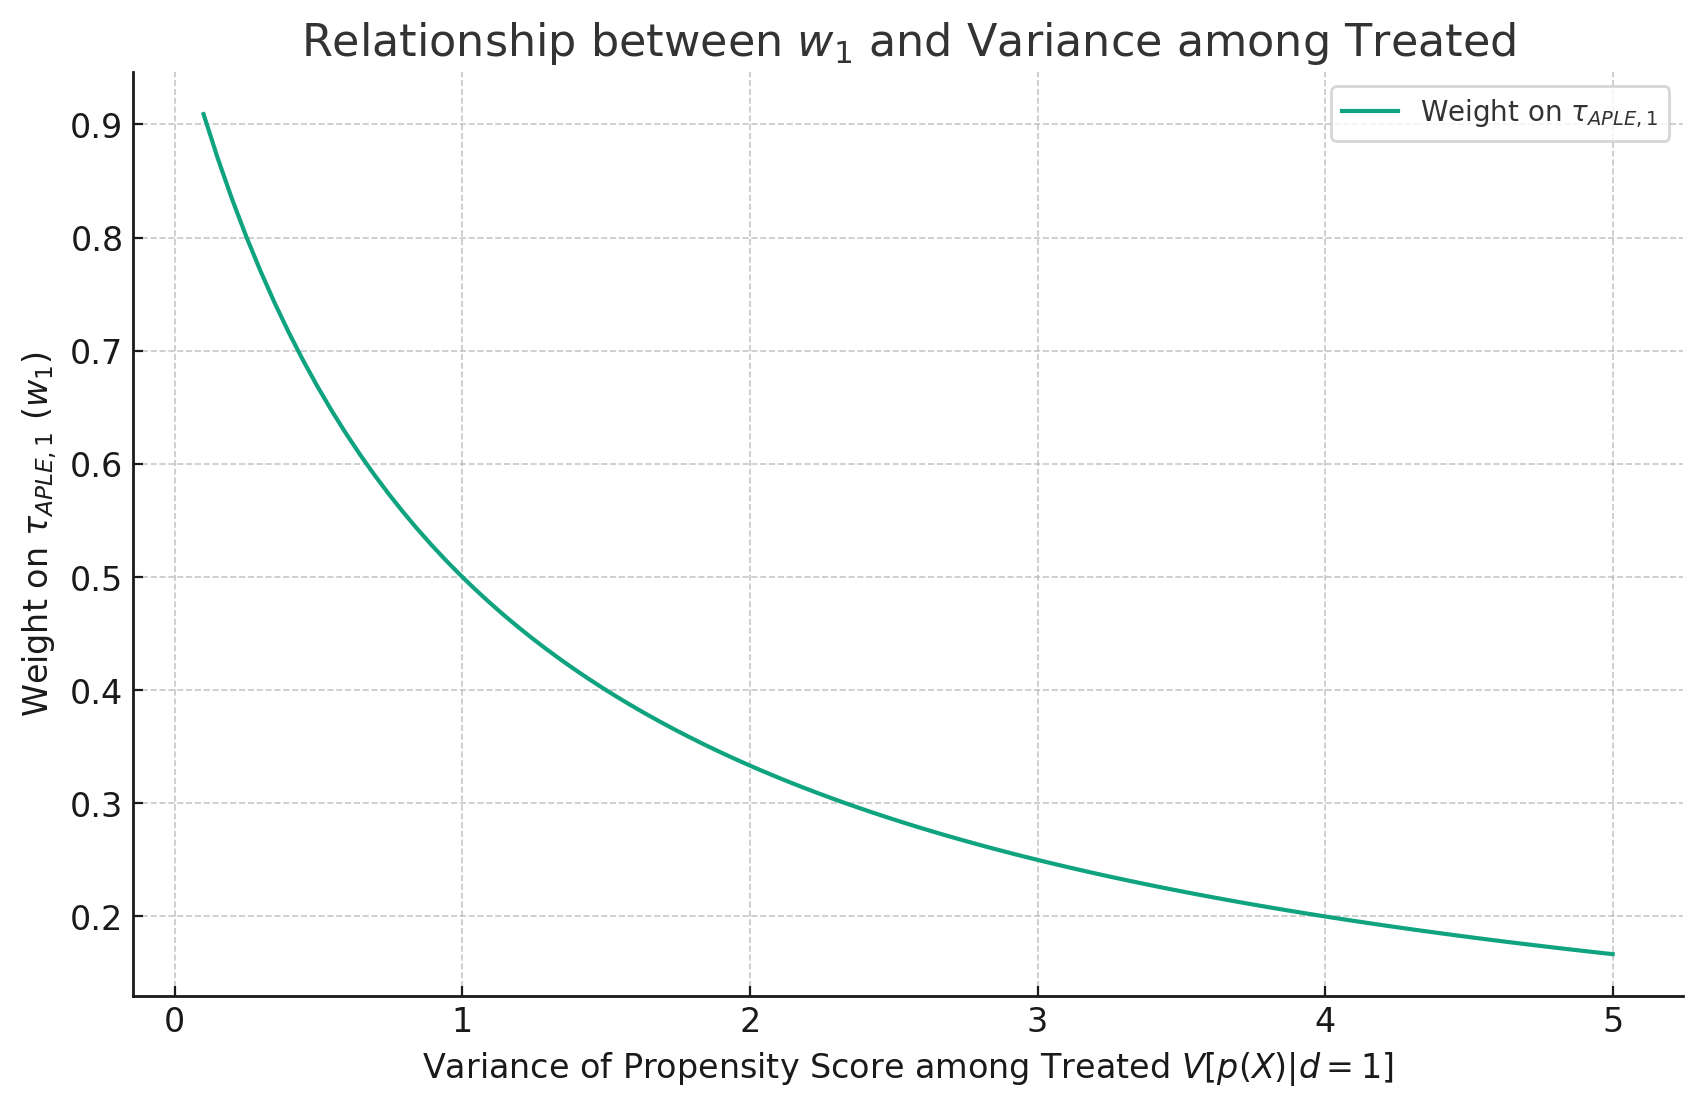
\includegraphics[width=0.8\textwidth]{./lecture_includes/tymon_variance_weight.png}
        \caption{The relationship between the weight \( \omega_1 \) on \( \tau_{\text{APLE},1} \) and the variance of the propensity score among the treated \( V[p(X) | d = 1] \). As the variance among the treated increases, the weight on \( \tau_{\text{APLE},1} \) decreases.}
    \end{figure}
\end{frame}

\begin{frame}{Causal Interpretation of OLS}
  Theorem 1 ("Weighted Average Interpretation of OLS") is general due to its reliance solely on the existence and uniqueness of linear projections; however, for a causal interpretation of OLS, we must introduce:
  \begin{itemize}
    \item Potential outcomes \( y(1) \) and \( y(0) \) instead of realized outcomes
    \item Defined causal parameters: ATE, ATT, and ATU
    \item Introduce assumptions that will ensure a causal interpretation of \( \tau \)
  \end{itemize}
\end{frame}

\begin{frame}{Assumption 3 for Causal Interpretation}
  \begin{block}{Unconfoundedness in Mean Potential Outcomes or "Ignorability in Means"}
    \begin{enumerate}
      \item \( E [y(1) | X, d] = E[y(1) | X] \)
      \item \( E[y(0) | X, d] = E[y(0) | X] \)
    \end{enumerate}
  \end{block}
  Assumptions 3 is our standard unconfoundedness assumption but limited to means (slightly weaker but it's all we need)
\end{frame}

\begin{frame}{Assumption 4 for Causal Interpretation}
  \begin{block}{Linearity in Potential Outcomes}
    Assumption 4 posits that the conditional expectations of potential outcomes are linear in the propensity score:
    \begin{enumerate}
      \item \( E[y(1) | X] = \alpha_1 + \gamma_1 \times p(X) \)
      \item \( E[y(0) | X] = \alpha_0 + \gamma_0 \times p(X) \)
    \end{enumerate}
  \end{block}
\end{frame}

\begin{frame}{Historical and Practical Context of Assumption 4}
  While not a common assumption, it is not necessarily strong due to:
  \begin{itemize}
    \item The flexibility in the specification of \( X \), which can include nonlinear terms.
    \item The automatic satisfaction of this assumption in saturated models.
  \end{itemize}

    The linearity assumption has historical roots and practical implications:
    \begin{itemize}
      \item Historically aligned with Rosenbaum and Rubin (1983).
      \item Assumed linearity of \( E[d | X] \) in several notable econometric works.
      \item It is restrictive but can be mitigated by model specification choices.
    \end{itemize}
\end{frame}

\begin{frame}[shrink]{Corollary 1: Causal Interpretation of OLS}
  Under assumptions the first two linear projection related assumptions and these two new causal assumptions, then
  \[
    \tau = \omega_1 \times \tau_{\text{ATT}} + \omega_0 \times \tau_{\text{ATU}}
  \]
  
  In words, this states that under those four assumptions, the OLS weights from theorem 1 apply to the causal parameters we care about, the ATT and the ATU, and so therefore $\tau$ has a causal interpretation.  
  
  \bigskip
  
  But there's a catch: the greater the proportion of treated units, the smaller the OLS weight on the ATT, which is a problem given ATE = $\rho \times ATT + (1-\rho) ATU$
\end{frame}

\begin{frame}[shrink]{Proving Corollary 1 with Assumptions 3 and 4}
  \begin{itemize}
    \item Assumption 3 (Unconfoundedness) allows us to estimate the ATE using realized outcomes, as the expected potential outcomes are equal to the observed outcomes conditional on covariates \( X \):
    \[ E[y(1) - y(0) | X] = E[y | X, d = 1] - E[y | X, d = 0] \]
    \item Assumption 4 specifies the functional form of the expected potential outcomes as linear in the propensity score:
    \[ E[y(1) | X] = \alpha_1 + \gamma_1 \times p(X), \quad E[y(0) | X] = \alpha_0 + \gamma_0 \times p(X) \]
    \item Together, they imply that the OLS estimand for the treated (\( \tau_{\text{ATT}} \)) and untreated (\( \tau_{\text{ATU}} \)) equates to the Average Partial Linear Effects (APLE):
    \[ \tau_{\text{ATT}} = \tau_{\text{APLE},1}, \quad \tau_{\text{ATU}} = \tau_{\text{APLE},0} \]
    \item This connects the causal treatment effects (ATT and ATU) directly to the estimated effects from the linear projections.
  \end{itemize}
\end{frame}
